
\section{Bayesian inference}

\frame{
\frametitle{Bayesian inference}

The posterior distribution of model parameters can be difficult to interpret.\newline
            
We want to \textbf{summarise} the information enclosed in these distribution.

}

%%%%%%%%%%%%%%%%%%%%%%%

\frame{
\frametitle{Point estimation}

Example: Arrival rate with $y=1$ and prior $\sim G(0.5,1)$.

\begin{figure}[!ht]
\centering
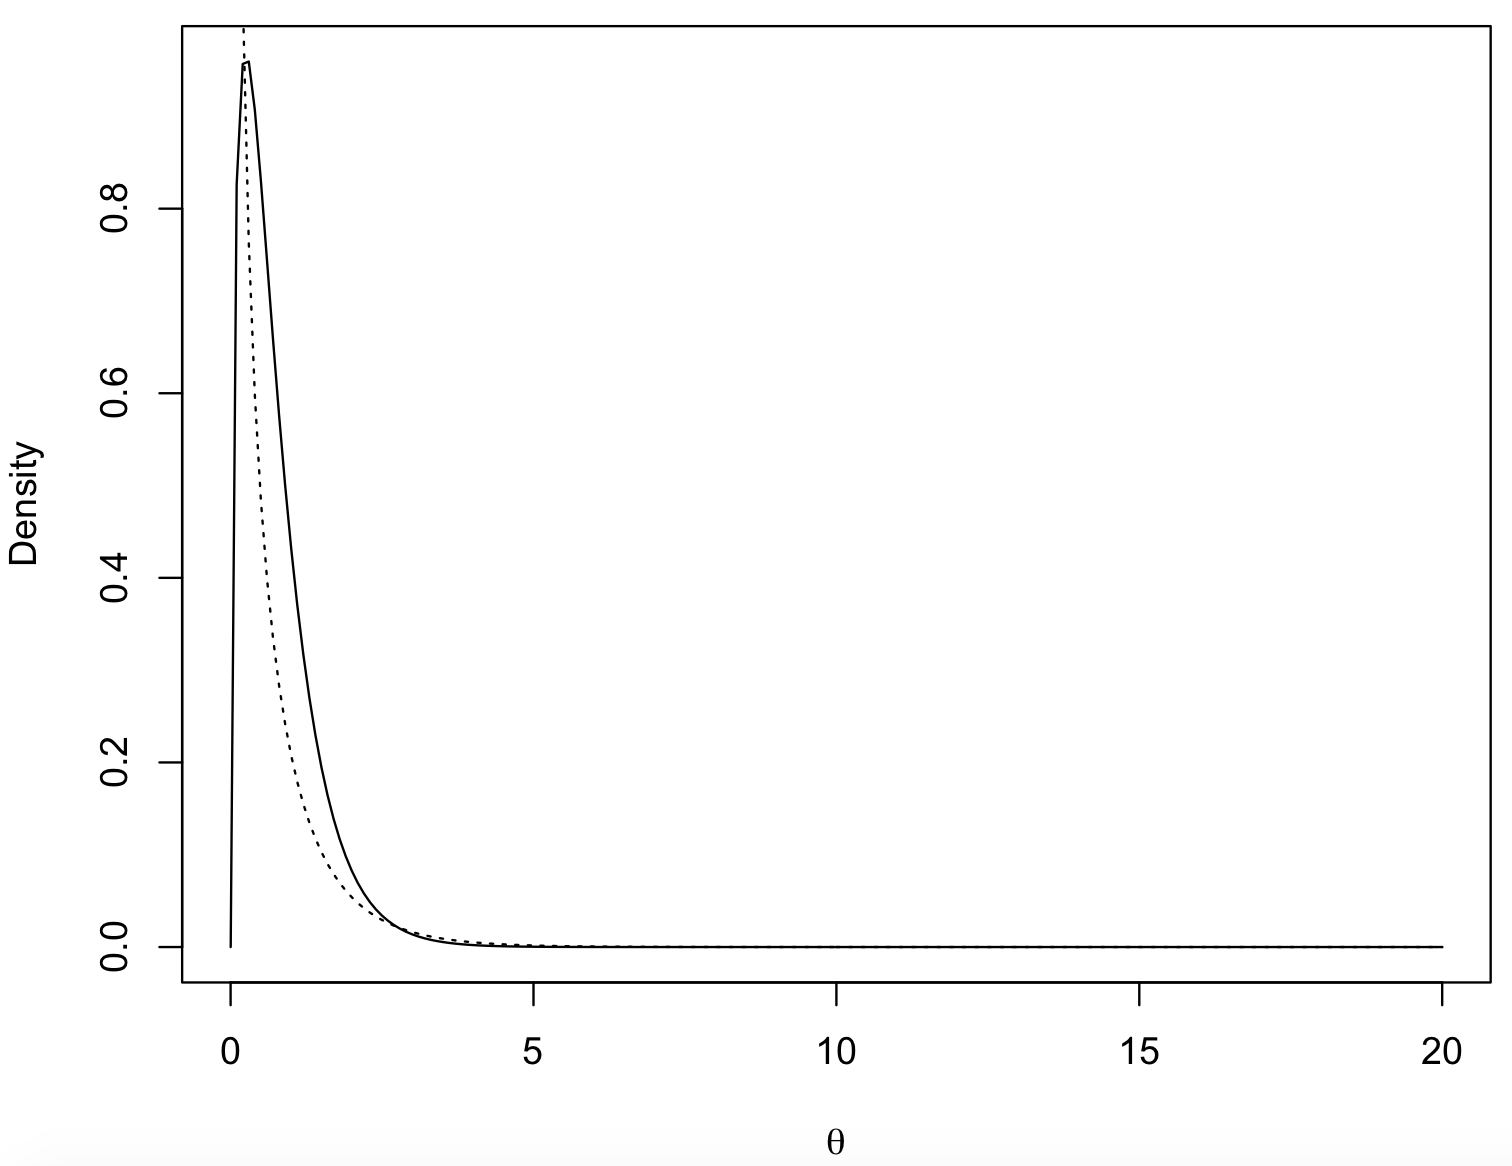
\includegraphics[width=5cm]{Figures/GammaSkewed.png}
%\caption{Posterior using a one-tailed gamma prior.}
\label{Fig:GammaSkewed}
\end{figure}

Question:\newline
What is the (i) mean, (ii) mode and (iii) median of this resulting posterior distribution?

}

%%%%%%%%%%%%%%%%%%%%%%%%%%%%%%%

\frame{
\frametitle{Point estimation}

\begin{itemize}
\item The mode is the easiest to calculate as we can work directly with the numerator.
\item If the prior distribution is flat then the \textit{posterior mode} will be equal to the maximum likelihood estimate.
\item If the posterior distribution is symmetric, then the mean and the median are equivalent.
\item For symmetric unimodal distributions, all these three features are equivalent.
\item For asymmetric distributions, the median is often the best choice as it is less affected by outliers and it is an intermediate to the mode and the mean.
\end{itemize}
       
}

%%%%%%%%%%%%%%%%%%%%%%%%%%%%%%%

\frame{
\frametitle{Point estimation}

If we want to obtain a measure of accuracy of a point estimate $\hat{\theta}(\vec{y})$, we can calculate the \textit{posterior variance}:

\begin{equation}
E_{\theta|\vec{y}}(\theta - \hat{\theta})^2 
\end{equation}

In the multivariate case the posterior mode is $\hat{\vec{\theta}}(\vec{y})=(\hat{\theta}_1,\hat{\theta}_2,...,\hat{\theta}_k)$.

}

%%%%%%%%%%%%%%%%%%%%%%%%%%%%%%%

\frame{
\frametitle{Credible intervals}

A $100 \times (1-\alpha)$ credible set for ${\theta}$ is a subset $C$ of ${\Theta}$ such that:
\begin{equation}
1-\alpha \leq P(C|{y}) = \int_C p({\theta}|{y})d{\theta}
\end{equation}

\textit{"The probability that $\theta$ lies in $C$ given the observed data $y$ is at least $(1-\alpha)$"}

e.g. $\alpha=0.05$

}

%%%%%%%%%%%%%%%%%%%%%%%%%%%%%%%

\frame{
\frametitle{Credible intervals}

In continuous settings we can calculate the \textit{highest posterior density}, or \textbf{HPD}, credible set, defined as:
\begin{equation}
C = \{ \theta \in \Theta : p(\theta|y) \geq k(\alpha) \}
\end{equation}
where $k(\alpha)$ is the largest constant satisfying $P(C|y)\geq(1-\alpha)$.\newline\newline

Example: $p(\theta|{y}) \sim G(2,1)$ and $k(\alpha)=0.1$.

}

%%%%%%%%%%%%%%%%%%%%%%%%%%%%%%%

\frame{
\frametitle{Credible intervals}

How can we summarise our results?
                \begin{itemize}
                \item the posterior mean
                \item several posterior percentiles (e.g. 0.025, 0.25, 0.50, 0.75, 0.975)
                \item a credible interval
                \item posterior probabilities $p(\theta>c|y)$ where $c$ is a notable point (e.g. 0, 1, depending on the problem)
                \item a plot of the distribution to check whether it is unimodal, multimodal, skewed, ...
                \end{itemize}

}

%%%%%%%%%%%%%%%%%%%%%%%%%%%%%%%

\frame{
\frametitle{Hypothesis testing}

In the \textbf{frequentist} approach,
\begin{enumerate}
\item one formulates a null hypothesis $H_0$ and an alternative hypothesis $H_a$,
\item an appropriate test statistic is chosen $T({Y})$,
\item one computes the \textit{observed significance}, or \textit{p-value}, of the test as the chance 
that $T({Y})$ is "more extreme" that $T({y}_{obs})$, where the "extremeness" is towards the alternate hypothesis,
\item if the p-value is less than some threshold, typically in the form of a pre-specified Type I error rate, $H_0$ is rejected, otherwise it is not.
\end{enumerate}

}

%%%%%%%%%%%%%%%%%%%%%%%%%%%%%%%

\frame{
\frametitle{Hypothesis testing}

Limits of frequentist approach:
\begin{enumerate}
\item only when two hypotheses are nested (e.g. $H_0$ is a simplification of $H_a$ and involves setting one parameter of $H_a$ to some known constant value)
\item evidence \textit{against} the null hypothesis (e.g. a large \textit{p}-value does not mean that the two models are equivalent, but only that we lack evidence of the contrary; we don't "accept the null hypothesis" but "fail to reject it")
\item no direct interpretation as weight of evidence (but only as a long-term probability; \textit{p}-values are not the probability that $H_0$ is true!)
\end{enumerate}

}

%%%%%%%%%%%%%%%%%%%%%%%%%%%%%%%

\frame{
\frametitle{Hypothesis testing}

In the \textbf{Bayesian} approach,
\begin{enumerate}
\item one can test as many models as desired, $M_i, i=1,...,m$,
\item one calculates the posterior probability that each model is correct
\item one compares each pair of posterior probabilities.
\end{enumerate}


}


%%%%%%%%%%%%%%%%%%%%%%%%%%%%%%%

\frame{
\frametitle{Hypothesis testing}

Suppose we have two models $M_1$ and $M_2$ for data $Y$ and the two models have parameters ${\theta}_1$ and ${\theta}_2$.

\vskip 1cm

With prior densities $\pi_i({\theta}_i)$ and $i=1,2$, the marginal distributions of $Y$ are:
                \begin{equation}
                p(y|M_i) = \int f(y|\theta_i,M_i) \pi_i(\theta_i) d\theta_i
                \end{equation}
\newline
We can calculate the posterior probabilities $P(M_1|y)$ and $P(M_2|y)=1-P(M_1|y)$ for the two models.

}

%%%%%%%%%%%%%%%%%%%%%%%%%%%%%%%

\frame{
\frametitle{Bayes factors}

A Bayes factor (BF) is used to summarise these results, and it is equal to the ration of posterior odds of $M_1$ to the prior odds of $M_1$:
                \begin{equation}
                BF = \frac{P(M_1|y)/P(M_2|y)}{P(M_1)/P(M_2)}=\frac{p(y|M_1)}{p(y|M_2)}
                \end{equation}
				
                If the two models are \textit{a priori} equally probable then:
                \begin{equation}
                BF = p(M_1|y) / p(M_2|y)
                \end{equation}
                which is the posterior odds of $M_1$.\newline
                
}

%%%%%%%%%%%%%%%%%%%%%%%%%%%%%%%

\frame{
\frametitle{Bayes factors}

\begin{block}{Interpretation}
BF captures the change in the odds in favour of model 1 (vs. 2) as we move from the prior to the posterior.
\end{block}

				\begin{table}[!ht]		
				\centering
				\label{Tab:BF}
				\begin{tabular}{c|c}
                \textbf{BF} & \textbf{Strength of evidence}\\
                1 to 3 & not worth more than a bare mention\\
				3 to 20 & positive\\
				20 to 150 & strong\\
   				$>150$ & very strong\\
				\end{tabular}
				\end{table}


}


%%%%%%%%%%%%%%%%%%%%%%%%%%%%%%%

\frame{
\frametitle{Practical 2: estimate population variation}

We now have sequenced our (bears') genomes and, using the method in Practical 1, assigned each individual genotype.

What is the frequency of a certain allele at the \textbf{population} level?

Follow instructions in the jupyter notebook.

}


